\documentclass[a4paper,10pt,twocolumn]{extarticle}
\usepackage[T1]{fontenc}
\usepackage[utf8]{inputenc}
\usepackage{geometry}
\geometry{margin=1.5cm,columnsep=0.65cm}
\usepackage{booktabs,graphicx,microtype,times}
\usepackage[font=small,labelfont=bf,skip=5pt]{caption}
\usepackage[hidelinks,breaklinks=true]{hyperref}
\usepackage{titlesec}
\titlespacing*{\section}{0pt}{9pt}{4pt}
\titleformat{\section}{\normalfont\large\bfseries}{\thesection.}{0.5em}{}
\raggedbottom
\begin{document}
\twocolumn[\begin{@twocolumnfalse}
\begin{center}
{\Large\bfseries Predictability Is Not Substitutability:\\
A Cost-of-Substitution Framework for H\&E-Based\\
Molecular Prediction Across 5 Cancers\par}
\medskip
{\small BIOINFO / GIW ISCB-Asia 2026 · Seoul, Korea · 17--20 November 2026 · Poster P082\par}
\medskip
Geongyu Lee\textsuperscript{1,2,*,\textdagger}, Ka-Kyung Kim\textsuperscript{1,*}, Sejin Park\textsuperscript{1,3}, Jaemyun Lyu\textsuperscript{1,4},\\
Jeong-Han Seo\textsuperscript{1,5,6}, Yong Gi Ji\textsuperscript{1,7}\par
\smallskip
{\small
\textsuperscript{1}Pseudo Lab, Republic of Korea; \textsuperscript{2}OmixAI Co. Ltd.; \textsuperscript{3}Seegene Inc.;
\textsuperscript{4}R\&D Center, Genolution Inc.;\\
\textsuperscript{5}ROKIT Genomics;
\textsuperscript{6}Department of Medical Science, University of Ulsan College of Medicine, Asan Medical Center;\\
\textsuperscript{7}Quantum C\&S\par
\smallskip
*Equal contribution. \textsuperscript{\textdagger}Corresponding author: \href{mailto:rjsrb365@gmail.com}{rjsrb365@gmail.com}\par}
\end{center}
\medskip
\end{@twocolumnfalse}]

\section{Introduction}

Deep learning models predict microsatellite instability, driver mutations and expression-based subtypes from H\&E histology, often with high reported accuracy \cite{kather2019,coudray2018,kather2020}. Discrimination metrics such as the area under the receiver operating characteristic curve (AUROC) measure how well a model separates molecular classes. However, replacing a molecular assay requires evaluating how prediction errors alter treatment assignment. Two models with the same AUROC can have different clinical consequences when their errors fall in different cells of the confusion matrix. Decision analysis has long separated discrimination from clinical consequence \cite{vickers2006}, yet studies of H\&E-based molecular prediction rarely extend this distinction to treatment routing.

In our prior work on early-stage breast cancer recurrence risk, an H\&E model achieved a sensitivity of 0.857 for the low-risk class but only 0.529 for the high-risk class \cite{lee2025}. The model missed roughly half of the high-risk patients who require escalated adjuvant treatment, showing that aggregate accuracy does not establish clinical substitutability. Moreover, histology-based biomarker predictions are vulnerable to site and cohort confounding across cancer types, datasets and model families \cite{dawood2026}. In a benchmark of 33 clinically actionable biomarker tasks, mean AUROC fell from 0.689 on internal data to 0.630 on an independent cohort \cite{goldmark2026}.

Here we present an endpoint-level framework to evaluate whether an H\&E model can substitute for a molecular test. A \textbf{treatment axis} is a treatment category: anti-HER2 therapy, endocrine therapy or chemotherapy. A \textbf{routing scheme} maps molecular labels to these axes. The \textbf{cost of substitution} measures the average therapeutic distance between reference and predicted assignments within each reference axis; the \textbf{misassignment rate} measures the fraction assigned to a wrong axis, without distance weighting. We combine this cost with an endpoint-level evidence protocol (site audit, shuffled null and a minimum number of hold-out positives) and apply it to TCGA cohorts from five cancers. The cost of substitution is computed in breast cancer, where treatment routing is defined; the evidence protocol is applied to every cohort.

\section{Methods}

We applied a single evaluation protocol across 5 cancer cohorts from The Cancer Genome Atlas (TCGA): breast (TCGA-BRCA, 1{,}010 patients), lung (1{,}050 patients), colorectal (534 patients), gastric (440 patients) and head and neck cancer (523 patients), with an endometrial extension (528 patients). Whole-slide images were segmented with Otsu thresholding and tiled at $256\times256$ pixels under $20\times$ magnification, with a cap of 5{,}000 tiles per slide. We extracted 1{,}024-dimensional tile embeddings using the UNI v1 foundation model \cite{chen2024} and aggregated them into patient-level scores using clustering-constrained attention multiple-instance learning (CLAM; single-branch CLAM-SB, or multi-branch CLAM-MB for multi-class subtype prediction) \cite{lu2021}. Cross-model analyses additionally used UNI2-h \cite{chen2024} and Virchow2 \cite{zimmermann2024}. Models were evaluated on a \textbf{site-disjoint hold-out} split, in which all slides from an institution were assigned exclusively to either training or evaluation.

We grouped cohorts into evidence classes based on when hold-out predictions were locked. In the \textbf{sealed-forward} lung, gastric and head and neck cohorts, predictions were sealed by version-control commit before hold-out results were produced (Table~1). The \textbf{anchor} breast cohort was used to develop the cost analysis; colorectal results were \textbf{retrospective}, meaning that results preceded sealing (Table~2). The endometrial extension was \textbf{exploratory}, meaning that it was analysed outside the sealed protocol. A \textbf{positive control} is an endpoint with established H\&E morphology used to check the pipeline. \textbf{Candidate endpoints} are the sealed-forward endpoints that are not positive controls; only these enter the confirmation tally. Early stopping used a development split taken from the training set; the validation and test sets were not used for model selection and are pooled as the hold-out. The breast anchor is the exception: its internal validation set was also used for checkpoint selection (Table~2). The pooled site-disjoint validation and test sets comprised 315 lung, 132 gastric and 157 head and neck hold-out patients.

Three diagnostic comparisons were applied to every endpoint: a 5-seed label-shuffled null distribution, a class-prevalence baseline and a shortcut baseline using either histological subtype alone or slide-level RGB pixel mean alone. Baselines are reported controls, not verdict rules, for all endpoints. An endpoint clears the shuffled null when its observed AUROC exceeds the null mean plus 2 standard deviations; confidence intervals use 1{,}000 bootstrap resamples (patients). With few positives, label-shuffled AUROCs vary widely, so this threshold can lie far above 0.5: for HPV under Virchow2, null AUROCs of 0.807, 0.214, 0.383, 0.262 and 0.543 gave a mean of 0.442, SD of 0.241 and threshold of 0.923. After modelling, a \textbf{site audit} was applied to 11 endpoints with site-level results: lung 3, gastric 4, head and neck 3, and colorectal BRAF V600E. The audit measured Cram\'er's $V$ between tissue-source site and label. The $V=1$ exclusion rule was applied following this audit, rather than fixed in advance.

\paragraph{Treatment routing and cost.} In the external breast cohort from the Clinical Proteomic Tumor Analysis Consortium (CPTAC-BRCA), primary \textbf{receptor routing} maps receptor status to an axis: HER2-positive to anti-HER2; otherwise ER-positive to endocrine; otherwise chemotherapy. \textbf{PAM50 routing} uses the PAM50 intrinsic subtype: HER2-enriched to anti-HER2, luminal A/B to endocrine and basal to chemotherapy. Slides with a reference Normal-like subtype are excluded; slides predicted Normal-like receive no treatment axis and are scored at the largest distance (0.765). A TCGA-BRCA model predicts ER and HER2 status (receptor routing) and a CLAM-MB model predicts the PAM50 subtype (PAM50 routing) for each CPTAC slide; ER and HER2 predictions are thresholded at the pre-specified 0.5 operating point and the PAM50 prediction is the highest-probability subtype; predicted and reference labels are routed by the same scheme. Receptor routing includes 294 slides from 95 CPTAC patients; PAM50 routing includes 382 slides from 115 patients. Per-axis costs and their contrast are computed over slides, with 95\% CIs from patient-cluster bootstrap resampling. For reference axis $a$, the cost of substitution is
\[
 C_a=\frac{1}{n_a}\sum_{i:a_i=a} d(a,\widehat a_i),
\]
where $n_a$ is the number of slides with reference axis $a$, $\widehat a_i$ is the routed axis and $d(a,a)=0$. \textbf{Therapeutic distance} is $d(a,b)=1-\tau_{ab}$, where Kendall's $\tau_{ab}$ compares the axes' drug-sensitivity rankings over 170 discriminating drugs using drug-response data from the Genomics of Drug Sensitivity in Cancer (GDSC2) resource, from 51 breast cancer cell lines. This distance is a proxy, not a measure of clinical harm. Distances are 0.395 for endocrine--anti-HER2, 0.695 for endocrine--chemotherapy and 0.765 for anti-HER2--chemotherapy. The corresponding misassignment rate is the fraction of these $n_a$ slides with $\widehat a_i\ne a$. The Yale HER2 trastuzumab cohort is an exploratory treatment-response cohort of 85 patients, including 36 responders, used to assess anti-HER2 prediction against pathological complete response (pCR).

\paragraph{Verdict scheme.} Sealed-forward candidate endpoints receive the first applicable verdict in this order:
\begin{enumerate}
\setlength{\itemsep}{0pt}
\item \textbf{Audit-excluded}: site and label are inseparable, with Cram\'er's $V(\mathrm{site},\mathrm{label})=1$; every institution contributes only one class.
\item \textbf{Undecided}: fewer than 25 hold-out positives.
\item \textbf{No signal}: the AUROC does not exceed the shuffled-null threshold.
\item \textbf{Confirmed}: the endpoint passes the preceding checks.
\end{enumerate}
The 25-positive threshold is a confirmatory-eligibility rule set without a power calculation; endpoints below it are reported as undecided rather than negative. Anchor, retrospective and exploratory endpoints receive the separate status \textbf{Not counted}. Positive controls are reported separately. A control passes if its hold-out AUROC clears the shuffled null under the primary model; when the null threshold exceeds 1 and the test is uninformative, the control fails if the 95\% CI of its AUROC includes 0.5. The site audit can exclude a control from interpretation. Baseline comparisons do not determine control pass/fail outcomes.

\begin{table*}[t]
\centering
\scriptsize
\caption{\textbf{Sealed-forward hold-out --- lung, gastric, head and neck.}
Cohorts in which predictions were sealed by commit before hold-out results were
produced; all 10 binary endpoints are listed, including three positive controls.}
\begin{tabular}{@{}lcccl@{}}
\toprule
\textbf{Endpoint} & \textbf{AUROC} & \textbf{95\% CI} & \textbf{Hold-out positives} & \textbf{Verdict} \\
\midrule
Head and neck HPV            & 0.959 & [0.921--0.986] & 26  & \textbf{Confirmed}\,$^\dagger$ \\
Gastric EBV & 0.948 & [0.861--1.000] & 7 & Undecided \\
Gastric MSI-H                & 0.860 & [0.759--0.941] & 24  & Undecided \\
Lung EGFR activating mutation & 0.852 & [0.725--0.953] & 15  & Undecided \\
Lung KRAS G12C               & 0.681 & [0.577--0.783] & 14  & Undecided \\
Gastric ERBB2 amplification  & 0.644 & [0.523--0.771] & 14  & Undecided \\
Head and neck EGFR amplification & 0.604 & [0.443--0.760] & 17 & Undecided \\
Lung LUSC histology (positive control) & 0.939 & [0.905--0.967] & 153 & Audit-excluded \\
Head and neck grade (positive control) & 0.815 & [0.742--0.882] & 41 & Control passed$^\ddagger$ \\
Gastric Lauren diffuse (positive control) & 0.536 & [0.379--0.694] & 31 & Control failed \\
\bottomrule
\end{tabular}

\vspace{2pt}
\begin{minipage}{0.92\textwidth}
\scriptsize $^\dagger$ Confirmed under UNI; with 20 label shuffles HPV cleared the null under all three models (see Results); limitations are summarised in the Discussion. $^\ddagger$ Control outcomes use UNI as the primary model; under UNI2-h, grade was 0.7469 against a null threshold of 0.7851.
\end{minipage}
\end{table*}
\begin{table}[t]
\centering
\scriptsize
\caption{\textbf{Anchor and retrospective cohorts --- breast and colorectal
(not counted).} Breast used internal validation predating the
cross-cancer protocol; this validation set was also used for checkpoint selection,
so no hold-out positive count is separately reported for it. Colorectal results were produced before the predictions were sealed and are
therefore retrospective; direction consistent with the framework does not make
them confirmatory. Colorectal anti-EGFR has 84 positives and is above the 25-positive eligibility threshold, but is excluded on status grounds. Colorectal MSI-H (21 positives) and colorectal BRAF V600E (15 positives) are below 25.}
\begin{tabular}{@{}lccl@{}}
\toprule
\textbf{Endpoint} & \textbf{AUROC} & \textbf{Hold-out positives} & \textbf{Status} \\
\midrule
Breast HER2             & 0.599 & ---  & Internal anchor \\
Colorectal anti-EGFR    & 0.705 & 84   & Retrospective \\
Colorectal MSI-H     & 0.918 & 21   & Retrospective \\
Colorectal BRAF V600E   & 0.882 & 15   & Retrospective \\
\bottomrule
\end{tabular}
\end{table}
\begin{figure}[t]
\centering
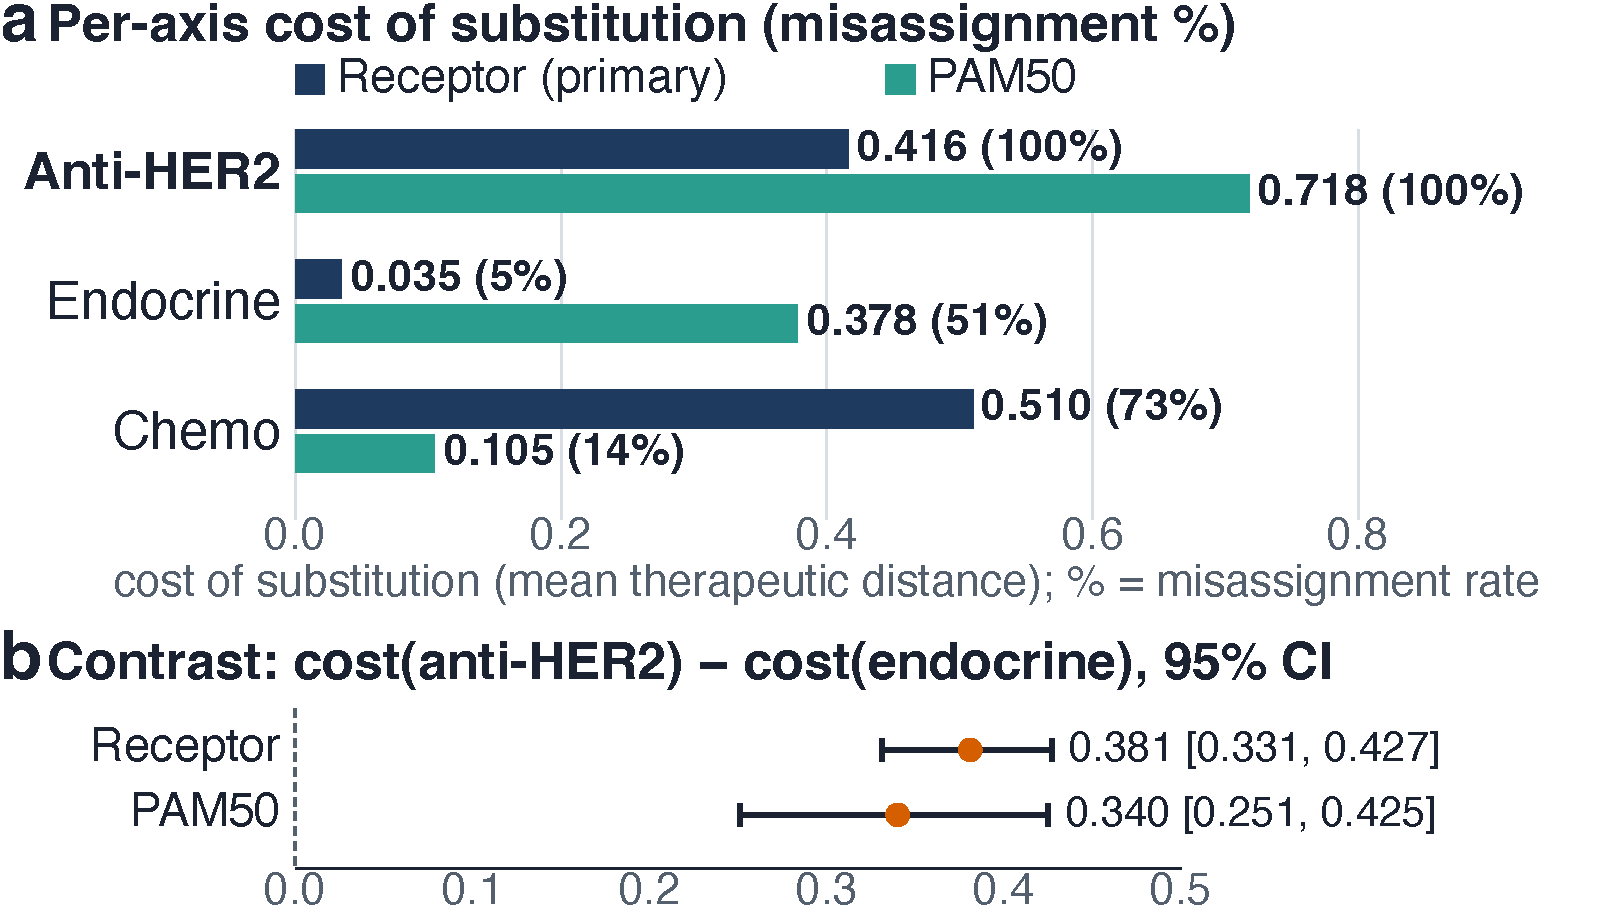
\includegraphics[width=\linewidth]{figures/fig_breast_cost.pdf}
\caption{\textbf{Cost of substitution in CPTAC-BRCA.} (a) Slide-level per-axis cost of substitution and misassignment percentages (receptor routing: 294 slides from 95 patients; PAM50 routing: 382 slides from 115 patients). Axes are anti-HER2 therapy, endocrine therapy and chemotherapy. Receptor routing maps HER2-positive to anti-HER2; otherwise ER-positive to endocrine; otherwise chemotherapy; PAM50 routing maps HER2-enriched, luminal A/B and basal subtype, respectively. Therapeutic distances ($1-\mathrm{Kendall}\ \tau$) are 0.395 for endocrine--anti-HER2, 0.695 for endocrine--chemotherapy and 0.765 for anti-HER2--chemotherapy. Anti-HER2 misassignment is 100\% under both schemes, with costs of substitution of 0.416 (receptor) and 0.718 (PAM50). Endocrine costs are 0.035 and 0.378; chemotherapy costs are 0.510 and 0.105, respectively. (b) Slide-level anti-HER2 minus endocrine contrasts with 95\% patient-cluster bootstrap CIs: 0.381 [0.331--0.427] and 0.340 [0.251--0.425], respectively. Both contrasts exclude 0.}

\end{figure}
\begin{figure}[t]
\centering
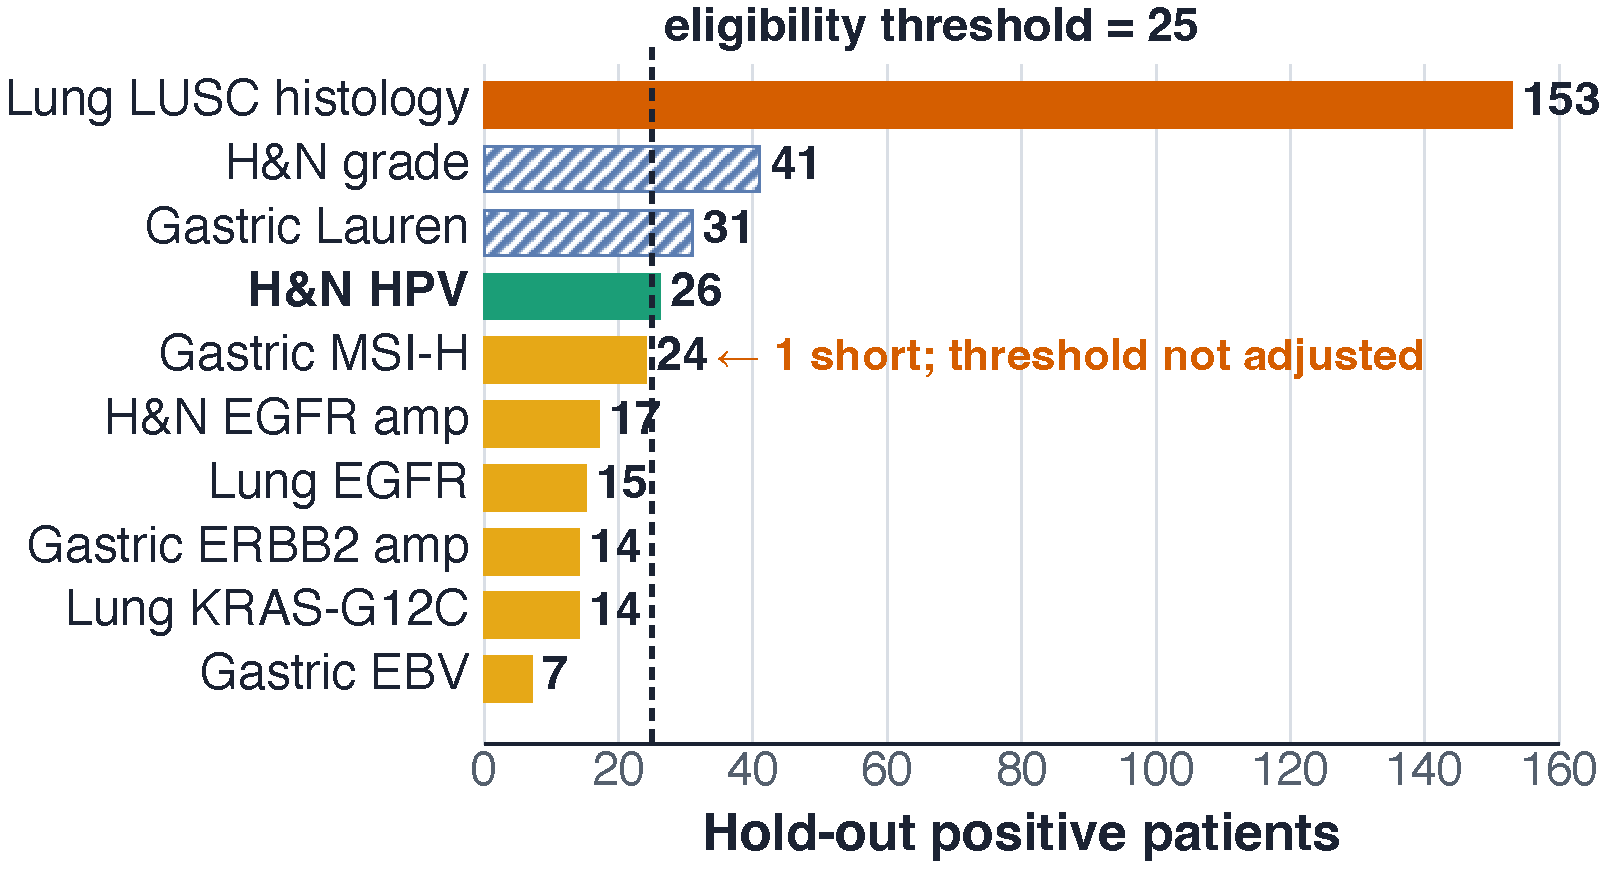
\includegraphics[width=\linewidth]{figures/fig_power_ceiling.pdf}
\caption{\textbf{The positive-count ceiling.} Hold-out positive counts per endpoint
against the confirmatory-eligibility threshold of 25 (dashed line). Colours mark verdicts: green, confirmed; orange, audit-excluded; amber, undecided. Hatched bars are positive controls (head and neck grade passed; gastric Lauren failed; lung histology was audit-excluded). Three of the four endpoints at or above the threshold are positive controls. All six non-HPV candidate endpoints fall below it and remain undecided.}
\end{figure}

\section{Results}

Of the 10 sealed-forward binary endpoints across lung, gastric and head and neck cancer, three served as positive controls: lung histology, gastric Lauren diffuse classification and head and neck grade. Among the seven non-control candidate endpoints, exactly one met the primary confirmation rule under the primary model (UNI): head and neck HPV; six remained undecided (gastric microsatellite instability-high, MSI-H; head and neck EGFR amplification, lung EGFR activating mutation, lung KRAS G12C, gastric ERBB2 amplification; gastric Epstein--Barr virus, EBV). Of the controls, head and neck grade passed, gastric Lauren failed and lung histology was audit-excluded. One further sealed prediction, that the terminal respiratory unit (TRU) subtype would be the best predicted of the lung transcriptomic subtypes, was inconclusive and is not tabulated. The breast and colorectal endpoints (Table~2) and the exploratory endometrial extension are reported separately and excluded from the confirmation tally.

\paragraph{Head and neck HPV.} Human papillomavirus (HPV) infection produces distinct histological features on H\&E, including non-keratinising and basaloid morphology. HPV association has been predicted from H\&E in oropharyngeal carcinoma \cite{klein2021}. HPV reached an AUROC of 0.959 [0.921--0.986] with 26 hold-out positives and met the confirmation rule under UNI. With 5 label shuffles it also cleared the null under UNI2-h and fell just below the threshold under Virchow2 (0.9199 vs 0.9234). In a later rerun with 20 shuffles, which stabilises the null, HPV cleared it under all three models (UNI 0.959 vs 0.789; UNI2-h 0.956 vs 0.730; Virchow2 0.920 vs 0.837). In a leave-one-site-out analysis with a logistic model on mean-pooled embeddings, HPV retained an AUROC of 0.840. Scores were stable under random tile dropout (score SD 0.0035 at 50\% dropout, no call changes).

\paragraph{Site-confounding audit.} Lung histological subtype classification—distinguishing lung adenocarcinoma (LUAD) from lung squamous cell carcinoma (LUSC)—reached an AUROC of 0.939, matching previously reported performance \cite{coudray2018}. However, the site audit revealed complete collinearity between institution and subtype label ($V(\mathrm{site},\mathrm{label}) = 1.000$), as TCGA institution codes coincided exactly with LUAD/LUSC status. Because site-specific digital histology signatures are a well-documented source of bias \cite{howard2021}, morphological signal could not be separated from institution effects, and the endpoint was audit-excluded. In a related shortcut comparison, the H\&E model for lung KRAS G12C reached an AUROC of 0.681, whereas predicting lung KRAS G12C from histological subtype alone reached 0.793. With 14 hold-out positives, lung KRAS G12C remained undecided; the histology-only baseline served as a diagnostic control rather than a verdict rule.

\paragraph{Gastric Lauren.} For gastric Lauren classification, the positive class was diffuse (including signet-ring), and 58 hold-out patients had Lauren labels. Performance dropped from a development AUROC of 0.963 (a 15\% development split held out from training for early stopping) to a hold-out AUROC of 0.536 (95\% CI 0.379--0.694, including 0.5). The pixel-mean baseline of 0.631 is reported as context. Positive prevalence was 46\% in training versus 53\% (31/58) in the pooled hold-out. A random split would have reported the development AUROC; the site-disjoint hold-out exposed the drop. The shuffled-null threshold exceeded 1.0 for UNI and Virchow2, so the null test is uninformative here, and the control fails because the 95\% CI of its hold-out AUROC includes 0.5. Because diffuse and signet-ring gastric carcinomas have classic H\&E morphology, this drop is consistent with a failure to generalise across institutions rather than with absent morphology.

\paragraph{Breast anchor.} In external CPTAC-BRCA, every slide whose reference axis was anti-HER2 was assigned to another axis under both routing schemes (misassignment rate 100\%). HER2 AUROC was 0.599 in TCGA internal validation and 0.530 in external CPTAC (slide level), but at the pre-specified 0.5 operating point no external CPTAC case was routed to anti-HER2. AUROC measures ranking across thresholds, whereas this misassignment rate describes the selected operating point. Costs of substitution differed despite equal misassignment (0.416 for receptor routing versus 0.718 for PAM50 routing) because slides were assigned to different axes: endocrine is therapeutically closer to anti-HER2 than chemotherapy. The endocrine and chemotherapy costs reversed in relative order between schemes, while the anti-HER2 minus endocrine contrast excluded 0 under both (Figure~1). In the exploratory Yale HER2 trastuzumab cohort ($n=85$; 36 responders), the anti-HER2 prediction yielded a pathological complete response (pCR) AUROC of 0.533 [0.411--0.653].

\paragraph{Positive counts.} All six non-HPV candidate endpoints had too few positive hold-out cases to meet the confirmatory-eligibility criterion (Figure~2). Hold-out positive counts were 15 for lung EGFR activating mutation, 14 for lung KRAS G12C, 14 for gastric ERBB2 amplification, 24 for gastric MSI-H, 7 for gastric EBV and 17 for head and neck EGFR amplification. Although gastric MSI-H fell just 1 patient short of the threshold, the eligibility rule was not adjusted.

\section{Discussion}

The protocol flagged three results that AUROC alone would have misrepresented: lung histology (0.939), whose label coincided with institution; gastric Lauren, which fell from 0.963 in development to 0.536 across institutions; and lung KRAS G12C (0.681), which a histology-only baseline exceeded (0.793). It also kept six endpoints with too few positives as undecided rather than negative. These findings show why evaluating clinical substitutability requires separating predictive discrimination, treatment misassignment and confirmatory eligibility. Although a site-disjoint split prevents slides of the same institution from spanning training and evaluation sets, strong associations between institution and label can still persist, as quantified across 11 endpoints in 4 cohorts. As a secondary robustness check that does not change verdicts, we repeated the null test with UNI2-h and Virchow2. Candidate-endpoint results other than HPV did not change: lung EGFR activating mutation, lung KRAS G12C, gastric MSI-H and gastric EBV cleared the null under all three. Gastric ERBB2 amplification did not clear the null under any model and head and neck EGFR amplification cleared it only under UNI2-h; both stay Undecided because they have fewer than 25 positives.

We evaluated MSI-H in endometrial cancer (TCGA-UCEC) as an exploratory extension outside the sealed protocol. Endometrial MSI-H met the eligibility criterion with 30 hold-out positives yet failed shuffled-null exclusion (AUROC 0.6236 against a threshold of 0.6710). One exploratory endpoint met the eligibility criterion and still failed the null, so small positive counts are not the only reason endpoints were not confirmed. Because the endometrial cohort was analysed outside the protocol, it is excluded from the confirmation tally.

These are observational, cohort-level results. For HPV, a pixel-mean baseline reached 0.922 [0.854--0.975], overlapping the model's CI; the label was moderately associated with site ($V=0.397$); the single HPV-positive patient with two slides received discordant scores (0.9226 and 0.0010); and region-level annotation is needed to distinguish tumour morphology from surrounding lymphoid stroma. In the breast anchor, broader operating-point analysis remains incomplete; the reported misassignment rate describes the pre-specified 0.5 threshold. The external pCR analysis provides an exploratory outcome check.

\section{Conclusion}

Recent studies have documented how confounding limits H\&E-based biomarker models \cite{dawood2026} and benchmarked their predictive performance across clinically actionable tasks \cite{goldmark2026}. Building on this work, our study introduces an evaluation protocol that applies four ordered verdicts to sealed-forward candidate endpoints: Audit-excluded, Undecided, No signal and Confirmed. Anchor, retrospective and exploratory endpoints are Not counted, and positive controls are reported separately. Among the seven sealed-forward non-control candidate endpoints, 1 was confirmed under UNI and six remained undecided below the eligibility criterion.

Explicitly reporting low-count endpoints as undecided preserves the distinction between insufficient evidence and a negative result, while the exploratory endometrial MSI-H analysis shows that meeting the eligibility criterion does not guarantee signal above the null. Together, cost-of-substitution weighting, site-confounding audits and eligibility rules that are explicit and applied identically provide a practical endpoint-level framework for evaluating H\&E models proposed as surrogates for molecular tests.

\section*{Code availability}
{\raggedright\url{https://github.com/Geongyu/predictability-substitutability}\par}

\section*{Acknowledgement}
This research was supported by the “Open Source AI·SW Developer and Community Support Program” funded by the Ministry of Science and ICT (MSIT), Republic of Korea. Conducted as an independent Pseudo Lab project; corporate affiliations are listed for identification only.

\begingroup
\scriptsize
\begin{thebibliography}{99}
\setlength{\itemsep}{0pt}

\bibitem{kather2019}
Kather JN \textit{et al.} Deep learning can predict microsatellite instability
directly from histology in gastrointestinal cancer.
\textit{Nat Med} 25:1054--1056 (2019).
\url{https://doi.org/10.1038/s41591-019-0462-y}

\bibitem{coudray2018}
Coudray N \textit{et al.} Classification and mutation prediction from
non--small cell lung cancer histopathology images using deep learning.
\textit{Nat Med} 24:1559--1567 (2018).
\url{https://doi.org/10.1038/s41591-018-0177-5}

\bibitem{kather2020}
Kather JN \textit{et al.} Pan-cancer image-based detection of clinically
actionable genetic alterations. \textit{Nat Cancer} 1:789--799 (2020).
\url{https://doi.org/10.1038/s43018-020-0087-6}

\bibitem{vickers2006}
Vickers AJ, Elkin EB. Decision curve analysis: a novel method for evaluating
prediction models. \textit{Med Decis Making} 26:565--574 (2006).
\url{https://doi.org/10.1177/0272989X06295361}

\bibitem{lee2025}
Lee G \textit{et al.} Assessing the risk of recurrence in early-stage breast
cancer through H\&E stained whole slide images. \textit{Sci Rep} 15:35069
(2025). \url{https://doi.org/10.1038/s41598-025-16679-x}

\bibitem{dawood2026}
Dawood M \textit{et al.} Confounding factors and
biases abound when predicting molecular biomarkers from histological images.
\textit{Nat Biomed Eng} (2026).
\url{https://doi.org/10.1038/s41551-026-01616-8}

\bibitem{goldmark2026}
Vanderbilt C \textit{et al.} GOLDMARK: Governed Outcome-Linked Diagnostic Model
Assessment Reference Kit. \textit{arXiv}:2603.20848 (2026).
\url{https://arxiv.org/abs/2603.20848}

\bibitem{klein2021}
Klein S \textit{et al.} Deep learning predicts HPV association in oropharyngeal
squamous cell carcinomas and identifies patients with a favorable prognosis
using regular H\&E stains. \textit{Clin Cancer Res} 27:1131--1138 (2021).
\url{https://doi.org/10.1158/1078-0432.CCR-20-3596}

\bibitem{howard2021}
Howard FM \textit{et al.} The impact of site-specific digital histology
signatures on deep learning model accuracy and bias.
\textit{Nat Commun} 12:4423 (2021).
\url{https://doi.org/10.1038/s41467-021-24698-1}

\bibitem{chen2024}
Chen RJ \textit{et al.} Towards a general-purpose foundation model for
computational pathology. \textit{Nat Med} 30:850--862 (2024).
\url{https://doi.org/10.1038/s41591-024-02857-3}

\bibitem{lu2021}
Lu MY \textit{et al.} Data-efficient and weakly supervised computational
pathology on whole-slide images.
\textit{Nat Biomed Eng} 5:555--570 (2021).
\url{https://doi.org/10.1038/s41551-020-00682-w}

\bibitem{zimmermann2024}
Zimmermann E \textit{et al.} Virchow2: scaling self-supervised mixed
magnification models in pathology. \textit{arXiv}:2408.00738 (2024).
\url{https://arxiv.org/abs/2408.00738}

\end{thebibliography}
\endgroup

\end{document}
